\documentclass[../main.tex]{subfiles}
 
\begin{document}

\subsection{Diffusion Equation}

\subsubsection{Introduction to Diffusion Equation}

\begin{equation}
    u_t - \mathrm{D} \, \Delta u = f \label{eq:d1}
\end{equation}
where $\Delta$ denotes the \textbf{Laplace Operator}:

\begin{equation}
    \Delta = \sum_{k=1}^n \, \frac{\partial^2}{\partial x_k^2} \label{eq:d2}
\end{equation}

When $f \equiv 0$, the equation is said to be \textbf{homogeneous} and in this case the \textbf{Superposition Principle} holds: if $u$ and $v$ are solutions of eq.\ref{eq:d1} and $a$, $b$ are real (or complex) numbers, $a \, u + b \, v$ also is a solution of eq.\ref{eq:d1}. More generally, if $u_k(\mathbf{x}, t)$ is a family of solutions depending on the parameter $k$ (integer or real) and $g = g(k)$ is a function rapidly vanishing at infinity, then
\begin{equation*}
    \sum_{k=1}^{\infty} \, u_k(\mathbf{x}, t) \, g(k) \quad \text{and} \quad \int_{- \infty}^{+ \infty} \, u_k(\mathbf{x}, t) \, g(k) \, \mathrm{d} k
\end{equation*}
are still solutions.

\subsubsection{General Diffusion Equation}

On the other hand eq.\ref{eq:d1} constitutes a much more general diffusion model, where by diffusion we mean, for instance, the transport of a substance due to the molecular motion of the surrounding medium. In this case, u could represent the concentration of a polluting material or of a solute in a liquid or a gas (dye in a liquid, smoke in the atmosphere) or even a probability density. We may say that the diffusion equation unifies at a macroscopic scale a variety of phenomena, that look quite different when observed at a microscopic scale.

Through eq.\ref{eq:d1} and some of its variants we will explore the deep connection between probabilistic and deterministic models, according (roughly) to the scheme:
\begin{equation*}
    \text{diffusion processes} \leftrightarrow \text{probability density} \leftrightarrow \text{differential equations}
\end{equation*}

The star in this field is Brownian motion, derived from the name of the botanist Brown, who observed in the middle of the 19th century, the apparently chaotic behavior of certain particles on a water surface, due to the molecular motion. This irregular motion is now modeled as a \textit{Stochastic Process} under the terminology of \textit{Wiener Process / Brownian Motion}. The operator
\begin{equation*}
    \frac{1}{2} \, \Delta
\end{equation*}
is strictly related to Brownian motion \footnote{In the theory of stochastic processes, $1/2 \, \Delta$ represents the \textit{infinitesimal generator of the Brownian motion}.} and indeed it captures and synthesizes the microscopic features of that process.

Under equilibrium conditions, that is when there is no time evolution, the solution u depends only on the space variable and satisfies the stationary version of the diffusion equation (letting $D = 1$):
\begin{equation}
    - \Delta u = f \label{eq:d3}
\end{equation}
($− u_{xx} = f$, in dimension $n = 1$). Eq.\ref{eq:d3} is known as the \textit{Poisson Equation}. When $f = 0$, it is called \textit{Laplace’s Equation} and its solutions are so important in so many fields that they have deserved the special name of \textbf{harmonic functions}. This equations will be considered in the next chapter.

\subsubsection{Heat conduction in a solid body}

\begin{SCfigure}[0.6][h!]
    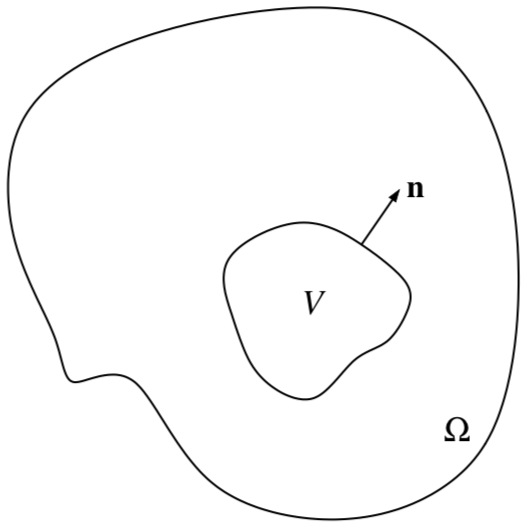
\includegraphics[width=0.4\textwidth]{Illustration_for_Basic_Law_of_Heat_Conduction}
    \caption{Illustration for Basic Law of Heat Conduction}
    \label{fig:d1}
\end{SCfigure}

A common example of diffusion is given by heat conduction in a solid body. Conduction comes from molecular collision, transferring heat by kinetic energy, without macroscopic material movement. If the medium is homogeneous and isotropic with respect to the heat propagation, the evolution of the temperature is described by eq.\ref{eq:d1}; $f$ represents the intensity of an external distributed source. For this reason eq.\ref{eq:d1} is also known as the \textbf{heat equation}.

Since heat is a form of energy, it is natural to use the law of conservation of energy, that we can formulate in the following way: Let $V$ be an arbitrary control volume inside the body. \textit{The time rate of change of thermal energy in $V$ equals the net flux of heat through the boundary $\partial V$ of $V$ , due to the conduction, plus the time rate at which heat is supplied by the external sources.}

If we denote by $e = e(\vec{x},t)$ the thermal energy per unit mass, the total quantity of thermal energy $M(t)$ and its time rate of change $M`(t)$ inside $V$ is given by:
\begin{align}
    M(t) &= \int_V \, \rho \, e(\vec{x},t) \, \mathrm{d} \vec{x} \\
    M`(t) &= \frac{\mathrm{d}}{\mathrm{d} t} \, \int_V \, \rho \, e(\vec{x},t) \, \mathrm{d} \vec{x} = \int \, \rho \, e_t(\vec{x},t) \, \mathrm{d} \vec{x}
\end{align}

\begin{equation}
    M`(t) = - \int_{\partial V} \, \vec{q}(\vec{x},t) \, \hat{\nu} \, \mathrm{d} \sigma + \int_V \, \rho \, r(\vec{x},t) \, \mathrm{d} \vec{x}
\end{equation}

Divergence theorem:
\begin{equation}
    M`(t) = - \int_{V} \, \nabla \vec{q}(\vec{x},t) \, \mathrm{d} \vec{x} + \int_V \, \rho \, r(\vec{x},t) \, \mathrm{d} \vec{x}
\end{equation}

Equation:
\begin{equation}
    \int \, \rho \, e_t(\vec{x},t) \, \mathrm{d} \vec{x} = - \int_{V} \, \nabla \vec{q}(\vec{x},t) \, \mathrm{d} \vec{x} + \int_V \, \rho \, r(\vec{x},t) \, \mathrm{d} \vec{x}
\end{equation}

The arbitrariness of $V$ allows us to convert the integral eq. into the pointwise relation:
\begin{equation}
    \rho \, e_t(\vec{x},t) = - \nabla \vec{q}(\vec{x},t) + \rho \, r(\vec{x},t)
\end{equation}

Final
\begin{equation}
    u_t - \frac{\kappa}{c_v \, \rho} \, \Delta u = \frac{1}{c_v} \, r
\end{equation}

\subsubsection{Well Posed Problems ($n = 1$)} \label{sec:2.1.3}

\begin{SCfigure}[0.6][h!]
    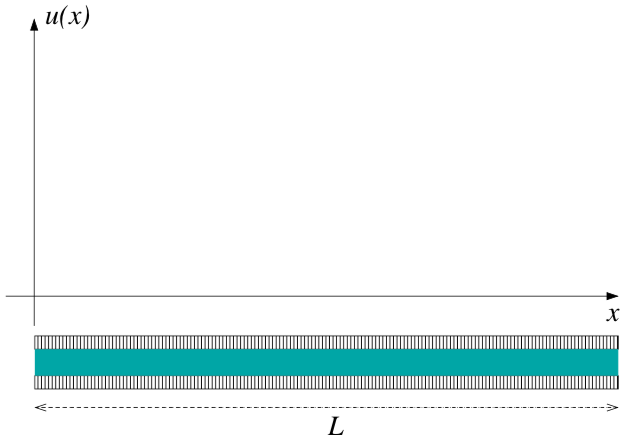
\includegraphics[width=0.4\textwidth]{Illustration_for_Heat_Conduction_in_a_Long_Bar}
    \caption{Illustration for Heat Conduction in a Long Bar}
    \label{fig:d2}
\end{SCfigure}

The problems associated with the above boundary conditions have a corresponding nomenclature. Summarizing, we can state the most common problems for the one dimensional heat equation as follows: given $f = f(x,t)$ (external source) and $g = g(x)$ (initial or Cauchy data), determine $u = u(x,t)$ such that:

\begin{align}
    \begin{cases}
        \, u_t - \mathrm{D} \, \Delta u = f & 0 < x < L \text{, } 0< t < T \\
        \, u(x,0) = g(x) & 0 \leqslant x \leqslant L \\
        \, \text{boundary condition} & 0 < t \leqslant T
    \end{cases}
\end{align}
where the boundary conditions may be: \\
    1. Dirichlet: $u(0,t) = h_1(t)$, $u(L,t) = h_2(t)$ \\
    2. Neumann: $- u_x(0,t) = h_1(t)$, $u_x(L,t) = h_2(t)$ \\
    3. Robin or Radiation: $- u_x(0,t) + \alpha \, u(0,t) = h_1(t)$, $u_x(L,t) + \alpha \, u(L,t) = h_2(t)$ \\
or mixed conditions. Accordingly, we have the initial-Dirichlet problem, the initial-Neumann problem and so on. When $h_1 = h_2 = 0$, we say that the boundary conditions are homogeneous.

\subsubsection{A solution by separation of variables} \label{sec:2.1.4}

\begin{quotebar}
    Mirza Karamehmedović: Many linear PDE problems can be solved using the so-called separation of variables that reduces the PDE problem to a set of ODE problems in the independent variables. This classical method dates back to Fourier (1812), who in fact developed what is now known as Fourier series to solve PDE problems.
\end{quotebar}

We will prove that, under reasonable hypotheses, the initial Dirichlet, Neumann or Robin and mixed problems are well posed. Sometimes this can be shown using elementary techniques like \textit{the separation of variables method} that we describe below through a simple example of heat conduction. \textcolor{red}{We emphasize that the reduction to homogeneous boundary conditions is crucial to carry on the computations.}

\begin{align}
    \begin{cases}
    \, U_t - \mathrm{D} U_{xx} = 0 \\
    \, U(x,0) = u^{st}(x) - g(x) \\
    \, U(0,t) = 0 \\
    \, U(L,t) = 0
    \end{cases}
\end{align}

Assume $U(x,t) = X(x) \, T(t)$, then
\begin{align}
    X \, T` - \mathrm{D} X`` \, T &= 0 \\
    \frac{T`}{\mathrm{D} \, T} - \frac{X``}{X} &= 0 \\
    \frac{1}{\mathrm{D}} \, \frac{T`(t)}{T(t)} = \frac{X``}{X} &= \lambda \quad \text{(constant) ???}
\end{align}

So, we get Eigen-Value Problem:
\begin{align}
    & X``(x) = \lambda \, X(x) \\
    & X(0) = X(L) = 0
\end{align}
and ODC ???
\begin{equation}
    T`(t) = \mathrm{D} \, \lambda \, T(t)
\end{equation}

To solve Eigen-Value Problem:

When we assume $\lambda > 0$:
\begin{align}
    & X(x) = \mathcal{C}_1 \, e^{\sqrt{\lambda} \, x} + \mathcal{C}_2 \, e^{- \sqrt{\lambda} \, x} \\
    & \begin{cases}
        \, X(0) = \mathcal{C}_1 + \mathcal{C}_2 = 0 \quad \text{and } \mathcal{C}_1 \neq 0 \text{, } \mathcal{C}_2 \neq 0 \\
        \, X(L) = \mathcal{C}_1 \, e^{\sqrt{\lambda} \, L} + \mathcal{C}_2 \, e^{- \sqrt{\lambda} \, L}
    \end{cases}
\end{align}

According to eq. :
\begin{align}
    & \mathcal{C}_2 (- e^{\sqrt{\lambda} \, L} + e^{- \sqrt{\lambda} \, L}) = 0 \\
    & - e^{\sqrt{\lambda} \, L} + e^{- \sqrt{\lambda} \, L} = 0 \\
    & \sqrt{\lambda} \, L = - \sqrt{\lambda} \, L \\
    & L = - L
\end{align}
This is not true, so the assumption of $\lambda > 0$ is wrong.

When we assume $\lambda = 0$:
\begin{align}
    & X``(x) = 0 \\
    & X(x) = \mathcal{C}_1 \, x + \mathcal{C}_2 \\
    & \begin{cases}
        \, X(0) = \mathcal{C}_2 = 0 \quad \mathcal{C}_1 \neq 0 \\
        \, X(L) = \mathcal{C}_1 \, L + \mathcal{C}_2 = \mathcal{C}_1 \, L = 0
    \end{cases}
\end{align}
This is not true, so the assumption of $\lambda = 0$ is wrong.

When we assume $\lambda < 0$, we set $\lambda = - \mu^2$, $\mu > 0$:
\begin{align}
    & X(x) = \mathcal{C}_1 \, \cos{(\mu \, x)} + \mathcal{C}_2 \, \sin{(\mu \, x)} \\
    & \begin{cases}
        X(0) = \mathcal{C}_1 = 0 \quad \text{and } \mathcal{C}_2 \neq 0 \\
        X(L) = \mathcal{C}_1 \, \cos{(\mu \, L)} + \mathcal{C}_2 \, \sin{(\mu \, L)} = \mathcal{C}_2 \, \sin{(\mu \, L)} = 0
    \end{cases}
\end{align}

So, we get:
\begin{align}
    & \sin{(\mu \, L)} = 0 \\
    & \mu_m \, L = m \, \pi \text{ ,  } m = 1 \text{, } 2 \text{, ...} \\
    & \mu_m = \frac{m \, \pi}{L} \text{ ,  } m = 1 \text{, } 2 \text{, ...} \\
    & \lambda_m = - \left(\frac{m \, \pi}{L}\right)^2 \text{ ,  } m = 1 \text{, } 2 \text{, ...}
\end{align}

So,
\begin{equation}
    X_m(x) = \mathrm{C}_2 \, \sin{\left(\frac{m \, \pi}{L} \, x\right)} \text{ ,  } m = 1 \text{, } 2 \text{, ...}
\end{equation}

And
\begin{align}
    & T`(t) = D \, \lambda \, T(t) = - \mu^2 \, D \, T(t) \\
    & T_m(t) = \mathcal{B} \, e^{- \mu_m^2 \, t} = \mathcal{B} \, e^{- \left(\frac{m \, \pi}{L}\right)^2 \, t} \text{ ,  } m = 1 \text{, } 2 \text{, ...}
\end{align}

And 
\begin{align}
    & U_m(x,t) = \mathcal{C}_2 \sin{\left(\frac{m \, \pi}{L} \, x\right)} \, \mathcal{B} \, e^{- \left(\frac{m \, \pi}{L}\right)^2 \, t} \text{ ,  } m = 1 \text{, } 2 \text{, ...} \\
    & U(x,t) = \sum_{m=1}^{\infty} \, \mathcal{A} \,  \sin{\left(\frac{m \, \pi}{L} \, x\right)} \, e^{- \left(\frac{m \, \pi}{L}\right)^2 \, t}
\end{align}

Then
\begin{align}
    & U(x,0) = u^{st}(x) - g(x) = \sum_{m=1}^{\infty} \, \mathcal{A} \, \sin{\left(\frac{m \, \pi}{L} \, x\right)} \, e^{- \left(\frac{m \, \pi}{L}\right)^2 \, t} \\
    & u(x,t) = u^{st}(x) - U(x,t) = u_0 + \frac{u_1 - u_0}{L} \, x - \sum_{m=1}^{\infty} \, \mathcal{A} \,  \sin{\left(\frac{m \, \pi}{L} \, x\right)} \, e^{- \left(\frac{m \, \pi}{L}\right)^2 \, t}
\end{align}

\textcolor{red}{Identify constants via initial condition, and validate the solution.}

\subsubsection{Problems in Dimension $n > 1$}

Summarizing, we have the following typical problems: given $f = f(\vec{x},t)$ and $g = g(\vec{x})$, determine $u = u(\vec{x},t)$ such that:
\begin{align}
    \begin{cases}
        \, u_t - \mathrm{D} \, \Delta \, u = f \quad \text{ in } Q_T \\
        \, u(\vec{x},0) = g(\vec{x}) \quad \text{ in } \overline{\Omega} \\
        \, \text{boundary conditions on } \partial \Omega \times (0,T]
    \end{cases}
\end{align}
where the boundary conditons could be:
\begin{enumerate}[nolistsep]
    \begin{easylist2}
        & Dirichlet: $u = h$
        & Neumann: $\partial_{\hat{\mu}} \, u = h$
        & Robin or Radiation: $\partial_{\hat{\mu}} \, u + \alpha \, u = h \quad (\alpha > 0)$
        & Mixed, for instance: $u = h_1 \text{ on } \Gamma_{\mathrm{D}}$, $\partial_{\hat{\mu}} \, u = h_2 \text{ on } \Gamma_{\mathrm{N}}$
    \end{easylist2}
\end{enumerate}

Also in dimension $n > 1$, the \textit{global Cauchy problem} is important:
\begin{align}
    \begin{cases}
        \, u_t - \mathrm{D} \, \Delta \, u = f \quad \vec{x} \in \mathbb{R}^n \text{ ,  } 0 < t < T \\
        \, u(\vec{x},0) = g(\vec{x}) \quad \vec{x} \in \mathbb{R}^n \\
        \, \text{conditions as } |\vec{x}| \rightarrow \infty
    \end{cases}
\end{align}

We again emphasize that no final condition (for $t = T$, $x \in \Omega$) is required. The data is assigned on the \textit{parabolic boundary} $\partial_p \, Q_T$ of $Q_T$ , given by the union of the bottom points $\overline{\Omega} 
\times {t=0}$ and the side points $S_T = \partial \Omega \times (0,T]$:
\begin{equation}
    \partial_p \, Q_T = (\overline{Q} \times {t=0}) \cup S_T
\end{equation}

\subsection{Uniqueness and Maximum Principle}

\begin{quotebar}
    Mirza Karamehmedović: Results regarding the existence and uniqueness of solution are essential in the analysis of PDEs. These results can tell us, e.g., whether a given model of a physical process is coherent and gives rise to a well-posed problem, and whether we should trust numerical solutions of the problem. The maximum principles that we shall consider are surprisingly strong and useful characterizations of solutions to the diffusion equation.
\end{quotebar}

\subsubsection{Integral method}

Generalizing the energy method used in Subsect. 2.1.4, it is easy to show that all the problems we have formulated in the previous section have at most one solution under reasonable conditions on the data. Suppose u and v are solutions of one of those problems, sharing the same boundary conditions, and let $w = u − v$; we want to show that $w \equiv 0$.

The above calculations are completely justified if $\Omega$ is a sufficiently smooth domain and, for instance, we require that $u$ and $v$ are continuous in $\overline{Q}_T = \overline{\Omega} \times [0,T]$, together with their first and second spatial derivatives and their first order time
derivatives. We denote the set of these functions by the symbol $C^{2,1} \, (\overline{Q}_T)$ and summarize everything in the following statement.

\textbf{Theorem 2.2}  The initial Dirichlet, Neumann, Robin and mixed problems have at most one solution belonging to $C^{2,1} \, (\overline{Q}_T)$.

\subsubsection{Maximum principles}

The fact that heat flows from higher to lower temperature regions implies that a solution of the homogeneous heat equation attains its maximum and minimum values on $\partial_p \, Q_T$. This result is known as the \textit{maximum principle} and reflects an aspect of the time irreversibility of the phenomena described by the heat equation, in the sense that the future cannot have an influence on the past (\textit{causality principle}). In other words, the value of a solution u at time t is independent of any change of the data after t.

\textbf{Definition 2.3}  A function $w \in C{2,1} (Q_T)$ such that $w_t − \mathrm{D} \, \Delta w \leqslant 0 (\geqslant 0)$ in $Q_T$ is called a sub-solution (super-solution) of the diffusion equation.

\textbf{Theorem 2.4}  Let $w \in C^{2,1} \, (Q_T) \cap C \, (\overline{Q}_T)$ such that ...

As an immediate consequence of Theorem 2.4, we have that, if
\begin{equation}
    w_t - \mathrm{D} \, \Delta w = 0 \quad \text{ in } Q_T
\end{equation}

then $w$ attains its maximum and its minimum on $\partial_p \, Q_T$. In particular,
\begin{equation}
    \min_{\partial_p \, Q_T} \, w \leqslant w(\vec{x}, t) \leqslant \max_{\partial_p \, Q_T} \, w \quad \text{ for every }(\vec{x},t) \in Q_T
\end{equation}

Moreover (for the proof see Problem 2.6):


\subsection{The Fundamental Solution}

\begin{quotebar}
    Mirza Karamehmedović: The fundamental solution is interesting since it is a special solution that can be used to construct other solutions.
\end{quotebar}

There are privileged solutions of the diffusion equation that can be used to construct many other ones. In this section we are going to discover one of these special building blocks, the most important one. First we point out some features of the heat equation.

\subsubsection{Invariant transformations}

\subsubsection{The fundamental solution ($n = 1$)}

Fundamental solution of $u_t - D \, \Delta u = 0$:
\begin{equation}
    \Gamma_D(x,t) = \frac{1}{\sqrt{4 \, \pi \, D \, t}} \, e^{- \frac{x^2}{4 \, D \, t}}
\end{equation}

\subsubsection{The Dirac distribution}

\subsubsection{The fundamental solution ($n > 1$)}

In space dimension greater than 1, we can more or less repeat the same arguments.

\subsection{The Global Cauchy Problem ($n = 1$)} \label{sec:2.8}

\begin{quotebar}
    Rasmus Dalgas Kongskov: Global Cauchy problem means that the equation is posed on the whole real line, i.e., not on a bounded domain. Since there are no boundaries in the traditional sense, the only data supplied is the initial condition.
\end{quotebar}

\subsubsection{The homogeneous case}

The global Cauchy problem:
\begin{equation}
    \begin{cases}
    u_t - \mathrm{D} u_{xx} = 0 \quad & \text{ in } \mathbb{R} * (0, \infty) \\
    u(x, 0) = g(x) \quad & \text{ in } \mathbb{R}
    \end{cases}
\end{equation}
where $g$, the \textit{initial datum}, is given.

Thanks to the linearity of the diffusion equation, we can use the superposition principle and compute the solution as the sum of all contributions. In this way, we get the formula:
\begin{equation}
    u(x,t) = \int_{\mathbb{R}} \, \Gamma_\mathrm{D}(x-y,t) \, g(y) \mathrm{d} y = \frac{1}{\sqrt{4 \, \pi \, \mathrm{D} \, t}} \, \int_{\mathbb{R}} \, e^{- \frac{(x-y)^2}{4 \,  \mathrm{D} \, t}} \, g(y) \, \mathrm{d} y 
\end{equation}

Clearly, one has to check rigorously that, under reasonable hypotheses on the initial datum $g$, eq.  really gives the unique solution of the Cauchy problem.

\subsubsection{Existence of a solution}

\textbf{Theorem 2.12}  Assume that there exist positive numbers $a$ and $c$ such that:
\begin{equation}
    |g(x)| \leqslant c \, e^{a \, x^2} \quad \text{ for all  } x \in \mathbb{R}
\end{equation}

Let $u$ be given by eq.2.135 and $T < \frac{1}{4 \, a \, D}$. Then the following properties hold.

\textbf{1)}  There are positive numbers $C$ and $A$ such that
\begin{equation}
    |u(x,t)| \leqslant C \, e^{A \, x^2} \quad \text{ for all  } (x,t) \in \mathbb{R} \times (0,T]
\end{equation}

\textbf{2)}  $u \in C ^{\infty} \, (\mathbb{R} \times (0,T])$ and in the strip $\mathbb{R} \times (0,T]$
\begin{equation}
    u_t - D \, u_{xx} = 0
\end{equation}

\textbf{3)}  Let $(x,t) \tightarrow (x_0,0^+)$. If $g$ is continuous at $x_0$ then $u(x,t) \rightarrow g(x_0)$

\textbf{Remark 2.13}  The theorem says that, if we allow an initial data with a controlled exponential growth at infinity expressed by eq.2.136, then eq.2.135 is a solution in the strip $\mathbb{R} \times (0,T)$. We will see that, under the stated conditions, eq.2.135 is actually the unique solution.

\subsubsection{Global maximum principles and uniqueness.}

The uniqueness of the solution to the global Cauchy problem is still to be discussed. This is not a trivial question since the following counterexample of Tychonov shows that there could be several solutions of the homogeneous problem.

Among the class of functions with growth at infinity controlled by an exponential of the type $C \, e^{A \, x^2}$ for any $t \geqslant 0$ (the so called Tychonov class), the solution to the homogeneous Cauchy problem is unique.

This is a consequence of the following maximum principle.

\textbf{Theorem 2.16 Global maximum principle}  Let $z$ be continuous in $\mathbb{R} \times [0,T]$, with derivatives $z_x$, $z_{xx}$, $z_t$ continuous in $\mathbb{R} \times (0,T)$, such that, in $\mathbb{R} \times (0,T)$:
\begin{align}
    & z_t - D \, z_{xx} \leqslant 0 \quad (\text{resp.} \geqslant 0) \nonumber \\
    & z(x,t) \leqslant C \, e^{A \, x^2} \quad \left(\text{resp.} \geqslant -e^{A \, x^2}\right)
\end{align}
where $C > 0$.

Then
\begin{equation}
    \sup_{\mathbb{R} \times [0,T]} \, z(x,t) \leqslant \sup_{\mathbb{R}} \, z(x,0) \quad \left(\text{resp.} \inf_{\mathbb{R} \times [0,T]} \, z(x,t) \geqslant \inf_{\mathbb{R}} \, z(x,0)\right)
\end{equation}

The proof is rather difficult \footnote{See [7], F. John, 1982.}, but if we assume that $z$ is bounded from above or below ($A = 0$ in (2.145)), then the proof relies on a simple application of the weak maximum principle, Theorem 2.4. In Problem 2.15 we ask the reader to fill in the details of the proof.

We now are in position to prove the following uniqueness result.

\textbf{Corollary 2.17 Uniqueness 1}  

\textbf{Corollary 2.18 Uniqueness 2}  Let $g$ be continuous in $\mathbb{R}$, satisfying eq.2.146, and let $f$ be as in Theorem 2.15. Then the Cauchy problem eq.2.144 has a unique solution $u$ in $\mathbb{R} \times [0,T]$, for $T < \frac{1}{4 \, D \, a}$, belonging to the Tychonov class. This solution is given by eq.2.135 and moreover
\begin{equation}
    \inf_{\mathbb{R}} + t \, \inf_{\mathbb{R} \times [0,T)} \, f \leqslant u(x,t) \leqslant \sup_{\mathbb{R}} \, g + t \, \sup_{\mathbb{R} \times [0,T)} \, f
\end{equation}

\subsubsection{Example of a homogeneous global Cauchy problem}

\begin{align}
    \begin{cases}
        \, u_t - 2 \, u_{xx} = 0 & \quad x \in \mathbb{R} \text{ ,  } t > 0 \\
        \, u(x,0) = g(x) = 4 \, e^{3 \, x^2} & \quad x \in \mathbb{R}
    \end{cases}
\end{align}

\textbf{Q1}  For what values of $x$ and $t$ are we guaranteed the existence and the uniqueness of a Tychonov-class solution of this problem?

\begin{equation}
    D = 2
\end{equation}

Assume that there exist positive numbers $a$ and $c$ such that:
\begin{equation}
    |g(x)| = 4 \, e^{3 \, x^2} \leqslant c \, e^{a \, x^2} \quad \text{ for all  } x \in \mathbb{R}
\end{equation}
Then $c = 4$, $a = 3$.

So we know from Theorem 2.12 that there is a unique solution:
\begin{equation}
    u(x,t) = \int_{\mathbb{R}} \, \Gamma_\mathrm{D}(x-y,t) \, g(y) \mathrm{d} y
\end{equation}
satisfies the estimate:
\begin{equation}
    |u(x,t)| \leqslant C \, e^{A \, x^2} \quad \text{ for all  } (x,t) \in \mathbb{R} \times (0,T]
\end{equation}
where $C$ and $A$ are positive numbers.

And therefore it belongs to the Tychonov class in $\mathbb{R} \times [0,T]$, for $T < \frac{1}{4 \, D \, a}$, according to Corollary 2.18.

\textbf{Q2}  Due to a measurement error, we are given the imperfect initial datum $\tilde{g}(x) = 4 \, e^{3 \, x^2} + e^{−|x|}$, $x \in \mathbb{R}$, instead of the correct initial datum $g$. For what values of $x$ and $t$ are we now guaranteed the existence and the uniqueness of a Tychonov-class solution of this problem?

Assume that there exist positive numbers $a_2$ and $c_2$ such that:
\begin{equation}
    \tilde{g}(x) = 4 \, e^{3 \, x^2} + e^{−|x|} \leqslant 4 \, e^{3 \, x^2} + 1 \leqslant 5 \, e^{3 \, x^2}
\end{equation}
Then $c_2 = 5$, $a_2 = 3$.

We can say the error in the initial data does not alter the domain for which the solution is of Tychonov class.

\textbf{Q3}  Let $u$ and $\tilde{u}$ be the unique Tychonov-class solutions of the above global Cauchy problem, with initial data $g$ and $\tilde{g}$, respectively. We keep the independent variables $x$ and $t$ in the domain where the solutions $u$ and $\tilde{u}$ exist and are unique. Estimate the maximal solution error $\sup_{x,t} \, |u(x,t) - \tilde{u}(x,t)|$ that can result due to the imperfect initial datum $g$?

Due to the linearity of the diffusion equation, the difference $z(x,t) = u(x,t) - \tilde{u}(x, t)$ leads to $z_t - D \, z_{xx} \leqslant 0$, but with $g_z(x) = g(x) - \tilde{g}(x) = - e^{-|x|}$. 

Since $z$ then is of Tychonov class, Theorem 2.12 shows that $z \in C^{\infty}(\mathbb{R} \times (0,T])$.

Then, according to Theorem 2.16:
\begin{equation}
    \sup_{x,t} \, |z(x,t)| \leqslant \sup_{x,t} \, |z(x,0)| = 1
\end{equation}

\subsection{An Example of Reaction-Diffusion in Dimension $n = 3$}

In this section we examine a model of reaction-diffusion in a fissionable material. Although we deal with a greatly simplified model, some interesting implications can be drawn.

By shooting neutrons into an uranium nucleus it may happen that the nucleus breaks into two parts, releasing other neutrons already present in the nucleus and causing a chain reaction. Some macroscopic aspects of this phenomenon can be described by means of an elementary model.

Suppose that a cylinder with height $h$ and radius $R$ is made of a fissionable material of constant density $\rho$. At a macroscopic level, the free neutrons diffuse like a chemical in a porous medium, with a flux proportional and opposite to its density gradient. In other terms, if $N = N (x, y, z,t)$ is the \textit{neutron density} and no fission occurs, the \textit{flux of neutrons is equal to} $− \kappa \, \Delta N$, where $\kappa$ is a positive constant depending on the material. The mass conservation law then gives $N_t - \kappa \, \Delta N = 0$. When fission occurs at a constant rate $\gamma > 0$, we get the \textit{reaction-diffusion equation} from eq.\ref{eq:d1}:
\begin{equation}
    N_t - \kappa \, \Delta N = \gamma \, N \label{eq:d5}
\end{equation}

We look for bounded solutions satisfying a homogeneous Dirichlet condition on the boundary of the cylinder, with the idea that the density is higher at the center of the cylinder and very low near the boundary. Then, it is reasonable to assume that N has a radial distribution with respect to the axis of the cylinder. More precisely, using the cylindrical coordinates $(r,\theta,z)$, of which the definition is in appendix, we write eq.\ref{eq:d5} to:
\begin{equation}
    N_t - \kappa \, [N_{rr} + \frac{1}{r} \, N_r + N_{zz}] = \gamma \, N \label{eq:d6}
\end{equation}

And, we can write $N = N(r,z,t)$ and the homogeneous Dirichlet condition on the boundary of the cylinder translates into:
\begin{align}
    \begin{split} \label{eq:d7}
        N(R, z, t) = 0 & \text{ ,  } \quad 0 < z < h \text{ ,  } \quad t > 0 \\
        N(r, 0, t) = N(r, h, t) = 0 & \text{ ,  } \quad 0 < r < R \text{ ,  } \quad t > 0 
    \end{split}
\end{align}

Accordingly we prescribe an initial condition
\begin{equation}
    N(r,z,0) = N_0(r ,z) \label{eq:d8}
\end{equation}
such that
\begin{align}
    \begin{split} \label{eq:d9}
        N_0(R, z) &= 0 \text{, } \quad 0 < z < h \\
        N_0(r, 0) &= N_0(r, h) = 0
    \end{split}
\end{align}

To solve problem of eq.\ref{eq:d6}, eq.\ref{eq:d7}, eq.\ref{eq:d8}, first we get rid of the reaction term by setting:
\begin{equation}
    N(r,z,t) = \mathcal{N}(r,z,t) \, e^{\gamma \, t} \label{eq:d10}
\end{equation}

By substituting eq.\ref{eq:d10} into eq.\ref{eq:d6}, we get:
\begin{align}
    (e^{\gamma \, t} \, \mathcal{N}_t + \gamma \, e^{\gamma \, t} \, \mathcal{N}) - \kappa \, [e^{\gamma \, t} \, \mathcal{N}_{rr} + \frac{1}{r} \, e^{\gamma \, t} \, \mathcal{N}_r + e^{\gamma \, t} \, \mathcal{N}_{zz}] &= \gamma \, e^{\gamma \, t} \, \mathcal{N} \nonumber \\
    \text{simplified to} \quad \mathcal{N}_t - \kappa \, [N_{rr} + \frac{1}{r} \, \mathcal{N}_r + \mathcal{N}_{zz}] &= 0 \label{eq:d11}
\end{align}
with the same initial and boundary conditions of $N$. So the problem becomes:
\begin{align}
    \begin{cases}
        \, \mathcal{N}_t - \kappa \, [\mathcal{N}_{rr} + \frac{1}{r} \, \mathcal{N}_r + \mathcal{N}_{zz}] = 0 \\
        \, \mathcal{N}_0(R, z) = 0 & \quad \text{ ,  } 0 < z < h \\
        \, \mathcal{N}_0(r, 0) = \mathcal{N}_0(r, h) = 0 & \quad \text{ ,  } 0 < r < R \\
        \mathcal{N}(R, z, t) = 0 & \quad \text{ ,  } 0 < z < h \text{ ,  } t > 0 \\
        \mathcal{N}(r, 0, t) = \mathcal{N}(r, h, t) = 0 & \quad \text{ ,  } 0 < r < R \text{ ,  } t > 0 
    \end{cases}
\end{align}

By maximum principle, we know that there exists only one solution, continuous up to the boundary of the cylinder. To find an explicit formula for the solution, we use the method of sepa- ration of variables, first searching for bounded solutions of the form:
\begin{equation}
    \mathcal{N}(r,z,t) = P(r) \, Z(z) \, T(t)
\end{equation}
satisfying the homogeneous Dirichlet conditions $u(R) = 0$ and $v(0) = v(h) = 0$.




\subsection{Appendix: Cylindrical Coordinates}

\begin{SCfigure}[0.6][h]
    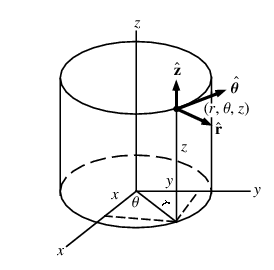
\includegraphics[width=0.4\textwidth]{Illustration_of_the_Cylinder_Coordinates}
    \caption{Illustration of the Cylinder Coordinates}
    \label{fig:ECBI1}
\end{SCfigure}

\FloatBarrier

\begin{align*}
    x = r \, \cos{\theta} \text{, } y = r \, \sin{\theta} \text{, } z = z \qquad (r > 0 \text{, } 0 \leqslant \theta \leqslant 2 \, \pi) \\
    \mathbf{e}_r = \cos{(\theta \, \mathbf{i})} + \sin{(\theta \, \mathbf{j})} \text{, } \mathbf{e}_{\theta} = - \sin{(\theta \, \mathbf{i})} + \cos{(\theta \, \mathbf{j})} \text{, } \mathbf{e}_z = \mathbf{k}
\end{align*}

Laplacian:
\begin{equation*}
    \begin{split}
        \Delta f &= \frac{1}{r} \frac{\partial}{\partial r} \left(r \, \frac{\partial f}{\partial r} \right) + \frac{1}{r^2} \frac{\partial^2 f}{\partial \theta^2} + \frac{\partial^2 f}{\partial z^2} \\
        &= \frac{\partial^2 f}{\partial r^2} + \frac{1}{r} \frac{\partial f}{\partial r} + \frac{1}{r^2} \frac{\partial^2 f}{\partial \theta^2} + \frac{\partial^2 f}{\partial z^2}
    \end{split}
\end{equation*}


\end{document}